\documentclass[]{article}

\usepackage{tabularx}
\usepackage[dutch]{babel}
\usepackage{amsmath}
\usepackage{graphicx}
\usepackage{amsmath}

\newcommand{\opgave}[1]{\section*{Opgave #1}}

\begin{document}

\opgave3
Alvorens de QR methode, al dan niet met shifts, toe te passen op de matrix, moeten we hem omzetten naar Hessenberg vorm. Deze omzetting kost ons \'{e}\'{e}nmaal \textit{O}($n^3$) rekenwerk. \linebreak
De QR factorisatie kan dan in \textit{O}($n^2$) berekend worden in plaats van in \textit{O}($n^3$). Dit moet in iedere iteratie van de QR methode uitgevoerd worden, dus  de vermindering in rekenwerk is erg significant. Daarbovenop komt dat de Hessenberg vorm al bijna bovendriehoeks is, waardoor  de QR factorisatie makkelijker (in minder stappen) uit te voeren is.

\begin{figure}
\begin{center}
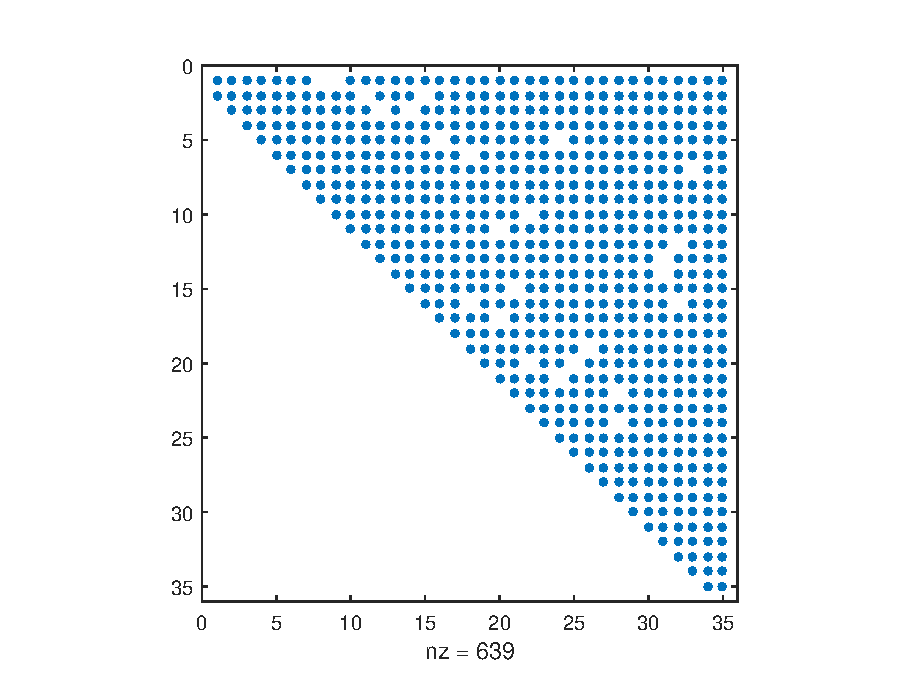
\includegraphics[width=1.4\textwidth]{opgave3.eps}
\end{center}
\caption{De structuur van de Hessenberg- vorm van mat1}
\end{figure}

\opgave4

De verwachting vanuit de theorie is dat de QR methode zonder shifts traag convergeert, zoals power- iteratie. De QR methode met shifts zou in het slechtste geval niet(Rayleigh shifts) of kwadratisch (Wilkinson shifts) convergeren.

Hieronder worden het benodigde aantal iteratiestappen per methode in grafiek- en tabelvorm weergegeven, samen met de fout op het tussenliggende resultaat. We merken op dat  zowel de Rayleigh Shift als de Wilkinson Shift zorgen voor een kubische convergentie (aantal beduidende cijfers \* 3 in iedere stap). 
De Wilkinson Shift heeft in dit geval een snellere convergentie door een (toevallig) goedgekozen eerste shiftwaarde. De convergentiefactor voor de eerste stap van de Wilkinson shift methode is hier $3.46$, voor de Rayleigh shift methode is hij $2.827$ en voor de QR methode zonder shift is hij zelfs kleiner dan 1. Het valt op dat de QR methode zonder shift niet lijkt te convergeren op deze grafiek. Dit is wel zo, maar pas na een groot aantal stappen (niet weergegeven). Na ~40 iteratiestappen is de machinenauwkeurigheid bereikt. 

\begin{figure}
\begin{center}
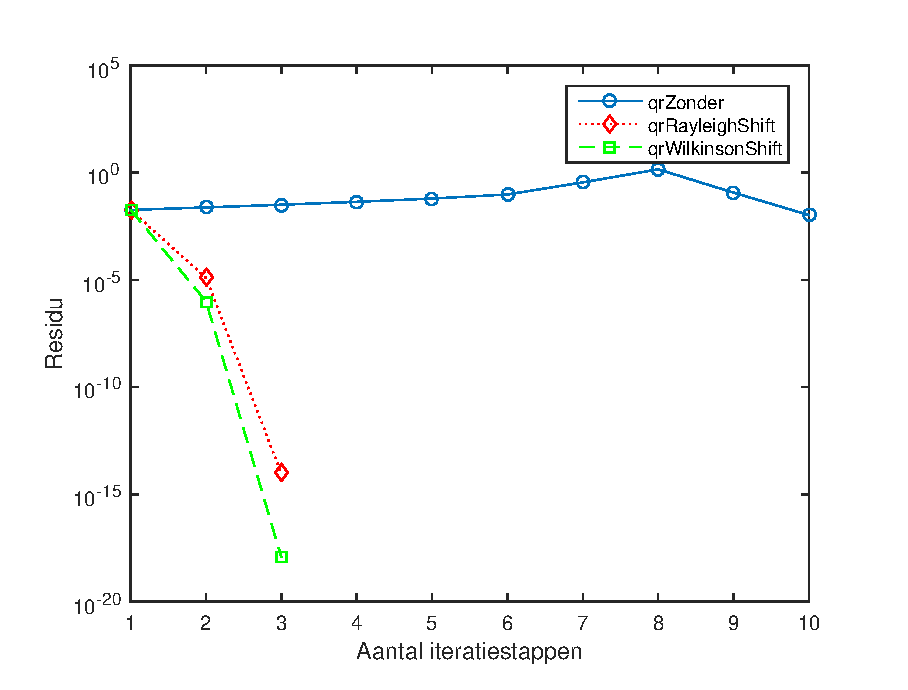
\includegraphics[width=1.4\textwidth]{opgave4.eps}
\end{center}
\caption{De fout op het berekenen van \'e\'en eigenwaarde.}
\label{figuurtje}
\end{figure}

\begin{table}
\noindent\makebox[\textwidth]{%
\begin{tabularx}{1.3\textwidth}{l|llllllllll}
methode&1&2&3&5&10&20&25\\\hline
qrZonder&$0.01836$ & $0.02411$ & $0.03212$ & $0.06223$ & $0.0106$ & $1.498\times 10^{-6}$ & $2.059\times 10^{-8}$ \\
qrRayleigh & $0.01836$ & $1.234\times 10^{-5}$ & $9.558\times 10^{-15}$\\
qrWilkinson & $0.01836$ & $9.833\times 10^{-7}$ & $1.138\times 10^{-18}$   \\
\end{tabularx}}
\caption{convergentie QR methodes voor eigenwaardenberekening}
\label{tabelOpgave4}
\end{table}


Een aantal zaken zijn nog op te merken:
\begin{itemize}
	\item Voor de 2 methoden die gebruik maken van shifts, wordt in iedere stap een aantal keren een geshifte inverse iteratie gedaan, om zo het element op positie $(k,k)$ te laten convergeren naar de $k-de$ eigenwaarde. Opmerkzaam is dat de $i-de$ eigenwaarde met $i = 1,\dots,k-1$ als k het aantal eigenwaarden is dat we nog moeten berekenen, ook al genaderd wordt, terwijl het algoritme nog bezig is eigenwaarden verderop in de matrix te berekenen m.b.v shift- iteraties. Hoe kleiner i, hoe minder sterk dit effect. De oorzaak hiervan is dat de QR methode, naast inverse iteratie, ook simultane iteratie toepast.
	\item De methode met Wilkinson- shifts doet er 66 stappen over om alle eigenwaarden van mat1 te vinden tot op machineprecisie. De methode met Rayleigh- shifts doet er 83 stappen over, en die zonder shifts maar liefst 686 stappen. Wilkinson shifts zijn beter dan de Rayleigh shifts, omdat zij rekening houden met het symmetrische eigenwaarden. Rayleigh shifts kunnen in zo'n gevallen zorgen voor een trage (of zelfs onbestaande) convergentie.
\end{itemize}

\end{document}
